\documentclass{article}

    \usepackage[tmargin=1in,lmargin=1in,rmargin=1in,bmargin=1in]{geometry}
    \usepackage[T1]{fontenc}
	\usepackage{titlesec}
	\usepackage{tikz}
    \usepackage{makecell}
    \usepackage{multicol}
    \usepackage{longtable}
	\usetikzlibrary{automata, positioning, arrows}
    \renewcommand{\familydefault}{\sfdefault}        	 
    \renewcommand\theadfont{\bfseries\sffamily}
    \tikzset{
        ->, % makes the edges directed
        >=stealth', % makes the arrow heads bold
        node distance=2cm, % minimum distance between two nodes. Change if necessary.
        every state/.style={thick, fill=gray!10}, % sets properties for each state node
        initial text=$ $, % sets the text that appears on the start arrow
    }
	\titleformat{\section}
	{\normalfont\bfseries}
	{\thesection.}{0.5em}{}
\begin{document}

\section*{Problem Set 1: Regular expressions and finite automata}
\begin{enumerate}
  \setlength\itemsep{-.25em}
  \item For strings containing the letters ‘a’, ‘b’, and ‘c’, give a regular expression that cap-tures all strings that have at least two (different, consecutive) letters in alphabetical order.
    \newline\newline
    \textbf{[a-c]*(ab|bc|ac)[a-c]*}  or  [a-c]*(ab|bc|ac)+[a-c]*
    \newline
    note: the plus is not necessary as the last regex captures all variations of the middle
    \newline
  \item Give a \textit{non-deterministic} finite automaton that captures the regular expression from
above. Show the automaton in graphical form.
  \newline
  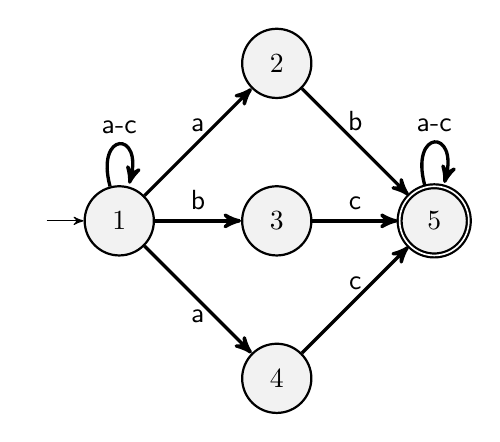
\begin{tikzpicture}
    \node[very thick, state, initial] (1) {$1$};
    \node[state, right of=1] (3) {$3$};
    \node[state, above of=3] (2) {$2$};
    \node[state, below of=3] (4) {$4$};
    \node[state, accepting, right of=3] (5) {$5$};
    \draw[very thick] (1) edge[loop above] node{a-c} (1)
          (1) edge[above] node{a} (2)
          (1) edge[left, above] node{b} (3)
          (1) edge[left, below] node{a} (4)
          (2) edge[left, above] node{b} (5)
          (3) edge[left, above] node{c} (5)
          (4) edge[left, above] node{c} (5)
          (5) edge[loop above] node{a-c} (5);
  \end{tikzpicture}
  \newline
  \item Using the construction described in class, give a \textit{deterministic} version of the automaton. You only need to show the transition table

      \begin{tabular}{|l|l|l|l|c|c|}
        \hline \thead{State} & \thead{a} & \thead{b} & \thead{c} & \thead{Final} & \thead{New Name}\\
        \hline 1			& 1, 2, 4		& 1, 3		& 1		& No	& 1\\
        \hline 1, 2, 4		& 1, 2, 4		& 1, 3, 5	& 1, 5	& No	& 2\\
        \hline 1, 3			& 1, 2, 4		& 1, 3		& 1, 5	& No	& 3\\
        \hline 1, 3, 5		& 1, 2, 4, 5	& 1, 3, 5	& 1, 5	& Yes	& 4\\
        \hline 1, 5			& 1, 2, 4, 5	& 1, 3, 5	& 1, 5	& Yes	& 5\\
        \hline 1, 2, 4, 5	& 1, 2, 4, 5	& 1, 3, 5	& 1, 5	& Yes	& 6\\
        \hline
      \end{tabular}
  \newline
  \newline
  \item Give a reduced version of the finite automaton, using the algorithm we used in class.You only need to show the state transition diagram.
    \begin{multicols}{2}
      \begin{tabular}{|l|l|l|l|c|}
        \hline \thead{State} & \thead{a} & \thead{b} & \thead{c} & \thead{Final}\\
        \hline 1	& 2		& 3		& 1		& No\\
        \hline 2	& 2		& 4		& 4		& No\\
        \hline 3	& 2		& 3		& 4		& No\\
        \hline 4	& 4		& 4		& 4		& Yes\\
        \hline
      \end{tabular}
 
    \begin{tikzpicture}
    \node[state, initial, below of=2, above of=3, left of=2] (1) {$1$};
    \node[state, above of=1, above of=3] (2) {$2$};
    \node[state, below of=1, below of=2] (3) {$3$};
    \node[state, accepting, above of=3, right of=3] (4) {$4$};
    \draw[very thick] (1) edge[loop above] node{c} (1)
          (1) edge[above] node{a} (2)
          (1) edge[left, above] node{b} (3)
          (2) edge[loop above] node{a} (2)
          (2) edge[right, above] node{b,c} (4)
          (3) edge[bend left, left] node{a} (2)
          (3) edge[right, below] node{b} (4)
          (3) edge[loop above] node{b} (3)
          (4) edge[loop above] node{a,b,c} (4);
    \end{tikzpicture}
    \end{multicols}
  \pagebreak
  \item Build a reduced, deterministic automaton for the following regular expression:
\[(a^*b^+c^+d^*)|(a^+b^*d^*)\]
    \begin{tikzpicture}
    \node[state, initial, below of=2, left of=2] (1) {$1$};
    \node[state, above of=1, above of=3] (2) {$2$};
    \node[state, right of=2] (3) {$3$};
    \node[state, right of=3] (4) {$4$};
    \node[state, accepting, right of=4] (5) {$5$};
    \node[state, below of=1, below of=2] (6) {$6$};
    \node[state, right of=6] (7) {$7$};
    \node[state, accepting, right of=7] (8) {$8$};
    \draw[very thick]
          (1) edge[above] node{} (2)
          (1) edge[above] node{a} (6)
          (2) edge[loop above] node{a} (2)
          (2) edge[right, above] node{b} (3)
          (3) edge[right, above] node{c} (4)
          (3) edge[loop above] node{b} (3)
          (4) edge[loop above] node{c} (4)
          (4) edge[right, above] node{} (5)
          (5) edge[loop above] node{d} (5)
          (6) edge[loop above] node{a} (6)
          (6) edge[right, above] node{} (7)
          (7) edge[loop above] node{b} (7)
          (7) edge[right, above] node{} (8)
          (8) edge[loop above] node{d} (8);
    \end{tikzpicture}
  \newline
  \newline
     \begin{tabular}{|l|l|l|l|l|c|c|}
        \hline \thead{State} & \thead{a} & \thead{b} & \thead{c} & \thead{d} & \thead{Final} & \thead{New Name}\\
        \hline 1, 2			& 2, 6, 7, 8	& 3			& err	& err	& No	& 1\\
        \hline 2, 6, 7, 8	& 2, 6, 7, 8	& 3, 7, 8	& err	& 8		& Yes	& 2\\
        \hline 3			& err			& 3			& 4, 5	& err	& No	& 3\\
        \hline 3, 7, 8		& err			& 3, 7, 8	& 4, 5	& 8		& Yes	& 4\\
        \hline 8			& err			& err		& err	& 8		& Yes	& 5\\
        \hline 4, 5			& err			& err		& 4, 5	& 5		& Yes	& 6\\
        \hline 5			& err			& err		& err	& 5		& Yes	& 7\\
        \hline
      \end{tabular}
  \newline
  \newline
  \newline
     \begin{tabular}{|l|l|l|l|l|c|c|}
        \hline \thead{State} & \thead{a} & \thead{b} & \thead{c} & \thead{d} & \thead{Final}\\
        \hline 1	& 2		& 3		& err	& err	& No\\
        \hline 2	& 2		& 4		& err	& 5		& Yes\\
        \hline 3	& err	& 3		& 6		& err	& No\\
        \hline 4	& err	& 4		& 6		& 5		& Yes\\
        \hline 5	& err	& err	& err	& 5		& Yes\\
        \hline 6	& err	& err	& 6		& 7		& Yes\\
        \hline 7	& err	& err	& err	& 7		& Yes\\
        \hline
     \end{tabular}
  \newline
  \newline
    \begin{tikzpicture}
    \node[state, initial, left of=2] (1) {$1$};
    \node[state, accepting, right of=1, below of=1] (2) {$2$};
    \node[state, above of=2, right of=1] (3) {$3$};
    \node[state, accepting, right of=2] (4) {$4$};
    \node[state, accepting, right of=4] (5) {$5$};
    \node[state, accepting, right of=3] (6) {$6$};
    \node[state, accepting, right of=6] (7) {$7$};
    \draw[very thick]
          (1) edge[above] node{a} (2)
          (1) edge[above] node{b} (3)
          (2) edge[loop above] node{a} (2)
          (2) edge[right, above] node{b} (4)
          (2) edge[bend right, below] node{d} (5)
          (3) edge[loop above] node{b} (3)
          (3) edge[right, above] node{c} (6)
          (4) edge[loop above] node{b} (4)
          (4) edge[right, above] node{d} (5)
          (4) edge[bend left, left] node{c} (6)
          (5) edge[loop above] node{d} (5)
          (6) edge[loop above] node{c} (6)
          (6) edge[right, above] node{d} (7)
          (7) edge[loop above] node{d} (7);
    \end{tikzpicture}
    \begin{tikzpicture}
    \node[state, initial, left of=2] (1) {$1$};
    \node[state, accepting, right of=1, below of=1] (2) {$2$};
    \node[state, above of=2, right of=1] (3) {$3$};
    \node[state, accepting, right of=2] (4) {$4$};
    \node[state, accepting, right of=4] (5) {$5$};
    \node[state, accepting, right of=3] (6) {$6$};
    \draw[very thick]
          (1) edge[above] node{a} (2)
          (1) edge[above] node{b} (3)
          (2) edge[loop above] node{a} (2)
          (2) edge[right, above] node{b} (4)
          (2) edge[bend right, below] node{d} (5)
          (3) edge[loop above] node{b} (3)
          (3) edge[right, above] node{c} (6)
          (4) edge[loop above] node{b} (4)
          (4) edge[right, above] node{d} (5)
          (4) edge[bend left, left] node{c} (6)
          (5) edge[loop above] node{d} (5)
          (6) edge[loop above] node{c} (6)
          (6) edge[right, above] node{d} (5);
    \end{tikzpicture}
\end{enumerate}
\end{document}

